\documentclass{article}
\usepackage[english]{babel}
\usepackage[utf8]{inputenc}
\usepackage[T1]{fontenc}
\usepackage{graphicx}
\usepackage{caption}
\usepackage{subcaption}
\usepackage{float}
\usepackage{wrapfig}
\usepackage{setspace}
\usepackage{cite}
\usepackage{url}
\usepackage{tikz}
\usetikzlibrary{positioning,trees}
\usepackage{soul}
\usepackage{color}
\definecolor{linkcol}{rgb}{0,0,0.4}
\definecolor{citecol}{rgb}{0.5,0,0}
\usepackage[pagebackref,hyperindex=true]{hyperref}
\hypersetup{colorlinks=true,linkcolor=linkcol,citecolor=citecol,urlcolor=linkcol}
\usepackage{xcolor}
\usepackage{listings}
%\lstset{
%	language=C++,
%	morekeywords={hsize_t},
%	keywordstyle=\color{blue},
%	commentstyle=\color{green},
%}

\lstdefinestyle{customc}{
  belowcaptionskip=1\baselineskip,
  breaklines=true,
  frame=L,
  xleftmargin=\parindent,
  language=C++,
  showstringspaces=false,
  basicstyle=\footnotesize\ttfamily,
  keywordstyle=\bfseries\color{blue!40!black},
  morekeywords={hsize_t},
  commentstyle=\itshape\color{purple!40!black},
  identifierstyle=\color{black},
  numberstyle=\color{red},
  stringstyle=\color{orange},
}

%\lstset{escapechar=@,style=customc}

\lstset{
language=C++,
basicstyle=\footnotesize\ttfamily,
keywordstyle=\bfseries\color{blue!60!black},
escapechar=@,
commentstyle=\itshape\color{purple!60!black},
showstringspaces=false,
morekeywords={hsize_t},
breaklines=true}


\begin{document}

\begin{titlepage}
\begin{center}
  \hfill
  \vspace{3.0cm}

  {\huge \textsc{IO Operations for wavepackets with HDF5 Interface in C++\\[10pt]
  }}
  ~\\[20pt]

  {\huge{Bachelor Thesis}}\\[2.5cm]

  {\emph{written by}}\\
  Florian Frei
  \\[0.6cm]
  {\emph{supervised by}}\\
  Dr. Vasile Gr\u{a}dinaru\\
  {\emph{and}}\\
  Prof. Dr. Ralf Hiptmair
  \\[2.5cm]

  Seminar for Applied Mathematics\\
  ETH Zurich
  \\[0.5cm]
  \emph{{Spring semester 2016}}
\end{center}
\end{titlepage}



\tableofcontents
\clearpage

\section{Introduction}
This thesis is about the continuation of the C++ implementation \cite{libwaveblocks} and allows a comparison to the Python implementation \cite{waveblocksnd}. The already existing framework is sufficient to generate simulations of different kind of Hagedorn wavepackets. The data produced is written in HDF5 binary format whereas the data from the C++ implementation is not easily comparable to the generated data from python. The writing process in the C++ implementation is currently done by using an extern project \cite{eigen3-hdf5}. The new implementation for writing binary HDF format in C++ will be explained in this thesis and also the new implementation allows easy comparison between Python and C++. It also incorporates a testing file which takes two HDF binary data files as arguments and compares the coinciding data. The testing file uses the well-known GoogleTest interface\cite{googletest}.

\section{HDF5 C++ Interface}
HDF stands for hierarchical data format which allows internal structure similar to a file system.
\subsection{Overview}
From the documentation we can conclude that the C++ interface is just a nice wrapper of the C interface. The corresponding classes and wrappers are shown in the following table:\\
\\
\begin{tabular}{|l|l|}
\hline
HDF5 C APIs&C++ Classes\\
\hline
Attribute Interface (H5A)&Attribute\\
Datasets Interface (H5D)&DataSet\\
Error Interface (H5E)&Exception\\
File Interface (H5F)&H5File\\
Group Interface(H5G)&Group\\
Identifier Interface (H5I)&IdComponent\\
Property List Interface (H5P)&PropList and subclasses\\
Dataspace Interface (H5S)&DataSpace\\
Datatype Interface (H5T)&DataType and subclasses\\
\hline
\end{tabular}\\
\\
The hierarchy of derivation of these classes is depicted in the following graph:\\
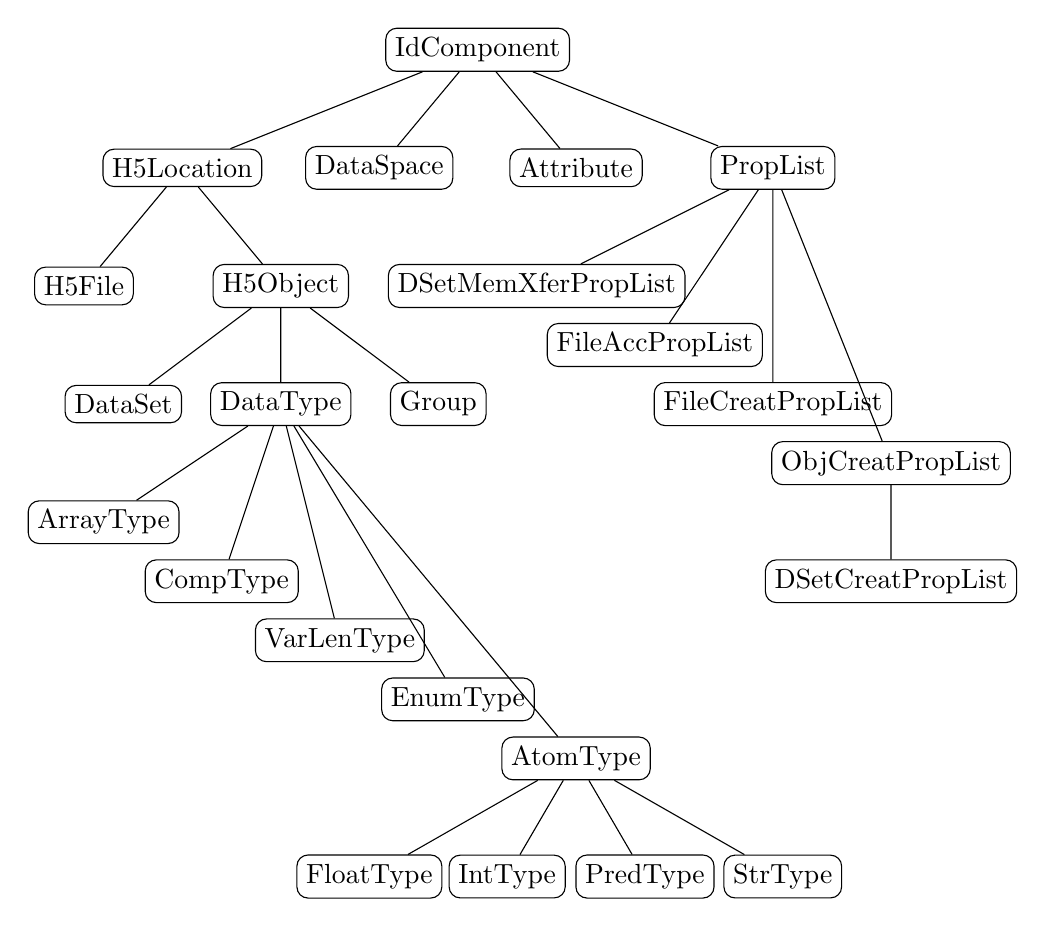
\begin{tikzpicture}[
baseline,
every node/.style = {shape=rectangle, rounded corners, draw, align=center},
]]
  \node {IdComponent}
    child[xshift=-1.5cm]
    {
        node{H5Location}
    	child[xshift=-0.5cm]{node{H5File}}
    	child[xshift=0.5cm]
    		{
    		node{H5Object}
    		child[xshift=-0.5cm]{node{DataSet}}
    		child{
    			node{DataType}
    			child[xshift=0.75cm]{node{ArrayType}}
    			child[xshift=0.75cm,yshift=-0.75cm]{node{CompType}}
    			child[xshift=0.75cm,yshift=-1.5cm]{node{VarLenType}}
    			child[xshift=0.75cm,yshift=-2.25cm]{node{EnumType}}
    			child[xshift=0.75cm,yshift=-3.0cm]
    				{
    				node{AtomType}
    				child[xshift=-0.375cm]{node{FloatType}}
    				child[xshift=-0.125cm]{node{IntType}}
    				child[xshift=0.125cm]{node{PredType}}
    				child[xshift=0.375cm]{node{StrType}} 
    				}
    			}
    		child[xshift=0.5cm]{node{Group}}
    		}
 	}
    child[xshift=-0.5cm]{node{DataSpace}}
    child[xshift=0.5cm]{node{Attribute}}
    child[xshift=1.5cm]{
    	node{PropList}
    	child[xshift=-0.75cm]{node{DSetMemXferPropList}}
    	child[xshift=-0.75cm,yshift=-0.75cm]{node{FileAccPropList}}
    	child[xshift=-0.75cm,yshift=-1.5cm]{node{FileCreatPropList}}
    	child[xshift=-0.75cm,yshift=-2.25cm]{
    		node{ObjCreatPropList}
    		child{node{DSetCreatPropList}}
    		}
    		};
\end{tikzpicture}\\


%Throughout this thesis we will ignore the "H5" namespace and will always directly refer to the name of the object.\\
For our purposes we need to save a \textit{Hagedorn} wave packet in every time step which consists of matrices and vectors. For these we need a \textit{DataSpace} which allows us to write matrices and vectors in a time-dimension. In our case the time-dimension is arbitrarily chosen depending on the kind of the simulation. As such we need a \textit{DSetCreatePropList} which is used to describe properties such as chunk-dimension for matrices used in our case for time-dimension.\textit{Attributes} are used to save additional information such as the used time-step $\delta t$ in the simulation. For constructing a HDF5 binary file we need to use the \textit{File} class which simply uses a string argument as the filename. For neatness we want to have a intern structure for our data. For this we use the \textit{Group} class which is very similar to the file system and its folders for structuring. To write \textit{Eigen}-matrices we need the \textit{DataType} class which defines how to write these data types. Last but not least we need a \textit{DataSet} for every object we want to write to our binary file.

\subsection{Intern used data-types}
Often we make function calls with arguments to the HDF5 library. These arguments have to be of an intern data type which the library expects. For our needs we mostly need hsize\_t and H5std\_string and every class mentioned in the previous section.
\subsubsection{hsize$\_$t}
Variables of this type represent native multiple-precision integer. 
\subsubsection{H5std$\_$string}
H5std\_string is just an alias for the std::string type.
\subsection{DataType}
The \textit{DataType} class describes how to write different kind of types and handles writing options. Every \textit{DataType} is given a name which is stored in a string used as its representation. As we can see from the previous graph \textit{DataType} is derived from \textit{H5Object} and is further decomposable in \textit{ArrayType}, \textit{AtomType}, \textit{CompType}, \textit{EnumType} and \textit{VarLenType}. For example when we want to write a native double and we don't care how it is represented on our system we would use a \textit{PredType} from \textit{AtomType} because it will use the definition from the operating system. When we would like to choose or define ourself how to write a double we would use the \textit{FloatType} from \textit{AtomType}. For cases where our data type is a struct of atomic types we would use the \textit{CompType}. For interested parties and further explanations we refer to the HDF5 official documentation\cite{hdf5doc}.
\subsection{DataSpace}
To write in a \textit{DataSet} the HDF5-library needs minimal four arguments. First is a pointer to the buffer of the source. Second is the type which is written which has to be a \textit{DataType} from before. Third and fourth is the source and destination space respectively which has to be a \textit{DataSpace} which will be explained in this section. There can be additional arguments such as which compression should be used for writing etc. A simple way to construct such a \textit{DataSpace} is to call the constructor with two arguments. The first one is the \textbf{rank} of the space, which indicates the number of dimension the space will have. Following as the second argument is an \textbf{array} of type \textbf{hsize\_t} with dimensionality of the previous declared \textbf{rank}. In each entry is the number of elements we want in this dimension. For example for a time grid \textit{DataSpace} the following code is sufficient:\\

\begin{lstlisting}
const int RANK = 1;
hsize_t size[RANK];
size[0]=number_of_timesteps;
\end{lstlisting}

The problem herein lies in the number of time steps which is unknown when we construct our \textit{DataSpace}. This leads to another approach which is to extend continuously which will be explained later on.
\subsection{DataSet}
A \textit{DataSet} is used as the location and representation for an object of interest which will be written. To construct a \textit{DataSet} we need four arguments. First argument is a string which represents the name and also the inner location in the file which will be explained later. The second argument describes the used \textit{DataType} to write data to this set. The third argument is a \textit{DataSpace} which describes the dimension of the \textit{DataSet}. The forth and last argument is a \textit{DSetCreatPropList} which describes inner properties of the DataSet for example the default fill value or the extensibility of the set.
\subsection{Attribute}
An \textit{Attribute} is used to write additional information to an existing \textit{Group} or \textit{DataSet} to describe the nature and/or the intended usage or the object. To create an \textit{Attribute} we need three arguments. First is a string for the name of the attribute. Second is the used \textit{DataType} of the \textit{Attribute}. Third and last is the \textit{DataSpace} of the attribute. In our case we want to add for example an \textit{Attribute} to the root \textit{Group} "/" which stores the time step used in this \textit{File}.
\subsection{DSetCreatePropList}
We use a \textit{DSetCreatPropList} to change the properties of how raw data is organized on disk and how the raw data is compressed. When default constructed a \textit{DataSet} is simple meaning it has fixed dimension but this doesn't allow us easy extension of the \textit{DataSet}. For this we change the property of how raw data is organized. When we define a chunk dimension for our data which is fixed we can easily extend the \textit{DataSet} later on in size of the chunk which also corresponds to a time step.
\subsection{Group}
We use \textit{Groups} to further structure our data in the file. Suppose we have a \textit{Hagedorn} wave packet and the corresponding energies with a time series then we would like to structure these in the file in a sub folder manner such as:
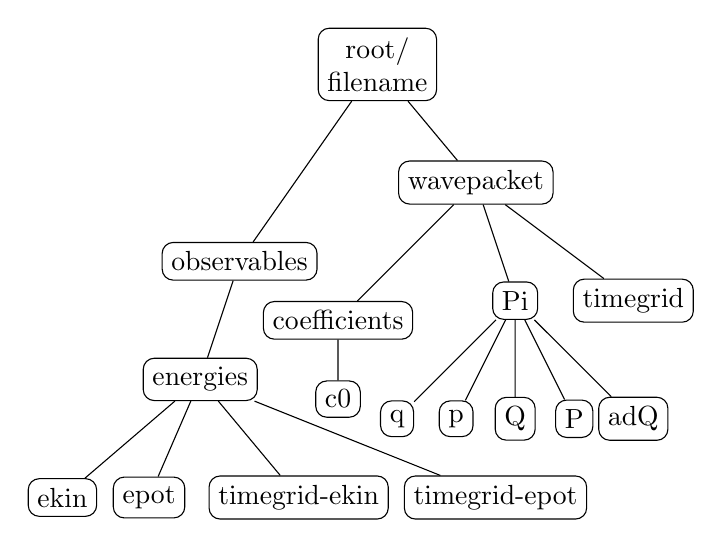
\begin{tikzpicture}[
baseline,
every node/.style = {shape=rectangle, rounded corners, draw, align=center},
]]
  \node {root/\\filename}
    child[yshift=-1cm,xshift=-1cm]
    {
    node{observables}
    child[xshift=-0.5cm]
            {
            node{energies}
    		child[xshift=0.5cm]{node{ekin}} 
    		child[xshift=0.1cm]{node{epot}}
    		child[xshift=0.5cm]{node{timegrid-ekin}}
    		child[xshift=1.5cm]{node{timegrid-epot}}
    		} 
    }
    child[xshift=0.5cm] 
    { 
    node {wavepacket}
    child[xshift=-0.25cm,yshift=-0.25cm]{node{coefficients}
    child[yshift=0.5cm]{node{c0}}}
    child[xshift=0.5cm]
    {
    node {Pi}
    child[xshift=1.5cm]{ node {q} }
    child[xshift=0.75cm] { node {p} }
    child { node {Q} }
    child[xshift=-0.75cm] { node {P} }
    child[xshift=-1.5cm] { node {adQ}}    
    }
    child[xshift=0.5cm]{node{timegrid}} 
	};
\end{tikzpicture}\\
This can be done with relatively easily when we use for every leaf a \textit{DataSet} and for every intermediate node a \textit{Group}. When a \textit{File} is created by default the root \textit{Group} has name "/" in the file. For enforcing the above structure one just needs to include the parents in the name during creation. For example the name for the coefficients \textit{Group} we would use "/wavepacket/coefficents" as name and for c0 \textit{DataSet} "/wavepacket/coefficents/c0".
\subsection{File}

\section{Eigen Interface}

\section{HDF5 Writer template}

\section{Datatest with GoogleTest Framework}
\subsection{Initialization}
\subsection{Testfissure}
\subsection{Testclass including HDF5 Interface}


%\nocite{*}


\bibliographystyle{plain}
\bibliography{references,wp,own}

\end{document}
